\documentclass{beamer}
\usepackage{amsmath,graphics}
\usepackage{amssymb}

\usetheme{default}
\usepackage{xcolor}

\definecolor{solarizedBase03}{HTML}{002B36}
\definecolor{solarizedBase02}{HTML}{073642}
\definecolor{solarizedBase01}{HTML}{586e75}
\definecolor{solarizedBase00}{HTML}{657b83}
\definecolor{solarizedBase0}{HTML}{839496}
\definecolor{solarizedBase1}{HTML}{93a1a1}
\definecolor{solarizedBase2}{HTML}{EEE8D5}
\definecolor{solarizedBase3}{HTML}{FDF6E3}
\definecolor{solarizedYellow}{HTML}{B58900}
\definecolor{solarizedOrange}{HTML}{CB4B16}
\definecolor{solarizedRed}{HTML}{DC322F}
\definecolor{solarizedMagenta}{HTML}{D33682}
\definecolor{solarizedViolet}{HTML}{6C71C4}
%\definecolor{solarizedBlue}{HTML}{268BD2}
\definecolor{solarizedBlue}{HTML}{134676}
\definecolor{solarizedCyan}{HTML}{2AA198}
\definecolor{solarizedGreen}{HTML}{859900}
\definecolor{myBlue}{HTML}{162DB0}%{261CA4}
\setbeamercolor*{item}{fg=myBlue}
\setbeamercolor{normal text}{fg=solarizedBase03, bg=solarizedBase3}
\setbeamercolor{alerted text}{fg=myBlue}
\setbeamercolor{example text}{fg=myBlue, bg=solarizedBase3}
\setbeamercolor*{frametitle}{fg=solarizedRed}
\setbeamercolor*{title}{fg=solarizedRed}
\setbeamercolor{block title}{fg=myBlue, bg=solarizedBase3}
\setbeameroption{hide notes}
\setbeamertemplate{note page}[plain]
\beamertemplatenavigationsymbolsempty
\usefonttheme{professionalfonts}
\usefonttheme{serif}

\usepackage{fourier}

\def\vec#1{\mathchoice{\mbox{\boldmath$\displaystyle#1$}}
{\mbox{\boldmath$\textstyle#1$}}
{\mbox{\boldmath$\scriptstyle#1$}}
{\mbox{\boldmath$\scriptscriptstyle#1$}}}
\definecolor{OwnGrey}{rgb}{0.560,0.000,0.000} % #999999
\definecolor{OwnBlue}{rgb}{0.121,0.398,0.711} % #1f64b0
\definecolor{red4}{rgb}{0.5,0,0}
\definecolor{blue4}{rgb}{0,0,0.5}
\definecolor{Blue}{rgb}{0,0,0.66}
\definecolor{LightBlue}{rgb}{0.9,0.9,1}
\definecolor{Green}{rgb}{0,0.5,0}
\definecolor{LightGreen}{rgb}{0.9,1,0.9}
\definecolor{Red}{rgb}{0.9,0,0}
\definecolor{LightRed}{rgb}{1,0.9,0.9}
\definecolor{White}{gray}{1}
\definecolor{Black}{gray}{0}
\definecolor{LightGray}{gray}{0.8}
\definecolor{Orange}{rgb}{0.1,0.2,1}
\setbeamerfont{sidebar right}{size=\scriptsize}
\setbeamercolor{sidebar right}{fg=Black}

\renewcommand{\emph}[1]{{\textcolor{solarizedRed}{\itshape #1}}}

\newcommand\dd{\mathrm d}
\newcommand\eul{\mathrm e}

\newcommand\cA{\mathcal A}
\newcommand\cB{\mathcal B}
\newcommand\cC{\mathcal C}
\newcommand\cD{\mathcal D}
\newcommand\cE{\mathcal E}
\newcommand\cF{\mathcal F}
\newcommand\cG{\mathcal G}
\newcommand\cH{\mathcal H}
\newcommand\cI{\mathcal I}
\newcommand\cJ{\mathcal J}
\newcommand\cK{\mathcal K}
\newcommand\cL{\mathcal L}
\newcommand\cM{\mathcal M}
\newcommand\cN{\mathcal N}
\newcommand\cO{\mathcal O}
\newcommand\cP{\mathcal P}
\newcommand\cQ{\mathcal Q}
\newcommand\cR{\mathcal R}
\newcommand\cS{\mathcal S}
\newcommand\cT{\mathcal T}
\newcommand\cU{\mathcal U}
\newcommand\cV{\mathcal V}
\newcommand\cW{\mathcal W}
\newcommand\cX{\mathcal X}
\newcommand\cY{\mathcal Y}
\newcommand\cZ{\mathcal Z}

\newcommand\fA{\mathfrak A}
\newcommand\fB{\mathfrak B}
\newcommand\fC{\mathfrak C}
\newcommand\fD{\mathfrak D}
\newcommand\fE{\mathfrak E}
\newcommand\fF{\mathfrak F}
\newcommand\fG{\mathfrak G}
\newcommand\fH{\mathfrak H}
\newcommand\fI{\mathfrak I}
\newcommand\fJ{\mathfrak J}
\newcommand\fK{\mathfrak K}
\newcommand\fL{\mathfrak L}
\newcommand\fM{\mathfrak M}
\newcommand\fN{\mathfrak N}
\newcommand\fO{\mathfrak O}
\newcommand\fP{\mathfrak P}
\newcommand\fQ{\mathfrak Q}
\newcommand\fR{\mathfrak R}
\newcommand\fS{\mathfrak S}
\newcommand\fT{\mathfrak T}
\newcommand\fU{\mathfrak U}
\newcommand\fV{\mathfrak V}
\newcommand\fW{\mathfrak W}
\newcommand\fX{\mathfrak X}
\newcommand\fY{\mathfrak Y}
\newcommand\fZ{\mathfrak Z}

\newcommand\fa{\mathfrak a}
\newcommand\fb{\mathfrak b}
\newcommand\fc{\mathfrak c}
\newcommand\fd{\mathfrak d}
\newcommand\fe{\mathfrak e}
\newcommand\ff{\mathfrak f}
\newcommand\fg{\mathfrak g}
\newcommand\fh{\mathfrak h}
%\newcommand\fi{\mathfrak i}
\newcommand\fj{\mathfrak j}
\newcommand\fk{\mathfrak k}
\newcommand\fl{\mathfrak l}
\newcommand\fm{\mathfrak m}
\newcommand\fn{\mathfrak n}
\newcommand\fo{\mathfrak o}
\newcommand\fp{\mathfrak p}
\newcommand\fq{\mathfrak q}
\newcommand\fr{\mathfrak r}
\newcommand\fs{\mathfrak s}
\newcommand\ft{\mathfrak t}
\newcommand\fu{\mathfrak u}
\newcommand\fv{\mathfrak v}
\newcommand\fw{\mathfrak w}
\newcommand\fx{\mathfrak x}
\newcommand\fy{\mathfrak y}
\newcommand\fz{\mathfrak z}

\newcommand\vA{\vec A}
\newcommand\vB{\vec B}
\newcommand\vC{\vec C}
\newcommand\vD{\vec D}
\newcommand\vE{\vec E}
\newcommand\vF{\vec F}
\newcommand\vG{\vec G}
\newcommand\vH{\vec H}
\newcommand\vI{\vec I}
\newcommand\vJ{\vec J}
\newcommand\vK{\vec K}
\newcommand\vL{\vec L}
\newcommand\vM{\vec M}
\newcommand\vN{\vec N}
\newcommand\vO{\vec O}
\newcommand\vP{\vec P}
\newcommand\vQ{\vec Q}
\newcommand\vR{\vec R}
\newcommand\vS{\vec S}
\newcommand\vT{\vec T}
\newcommand\vU{\vec U}
\newcommand\vV{\vec V}
\newcommand\vW{\vec W}
\newcommand\vX{\vec X}
\newcommand\vY{\vec Y}
\newcommand\vZ{\vec Z}

\newcommand\va{\vec a}
\newcommand\vb{\vec b}
\newcommand\vc{\vec c}
\newcommand\vd{\vec d}
\newcommand\ve{\vec e}
\newcommand\vf{\vec f}
\newcommand\vg{\vec g}
\newcommand\vh{\vec h}
\newcommand\vi{\vec i}
\newcommand\vj{\vec j}
\newcommand\vk{\vec k}
\newcommand\vl{\vec l}
\newcommand\vm{\vec m}
\newcommand\vn{\vec n}
\newcommand\vo{\vec o}
\newcommand\vp{\vec p}
\newcommand\vq{\vec q}
\newcommand\vr{\vec r}
\newcommand\vs{\vec s}
\newcommand\vt{\vec t}
\newcommand\vu{\vec u}
\newcommand\vv{\vec v}
\newcommand\vw{\vec w}
\newcommand\vx{\vec x}
\newcommand\vy{\vec y}
\newcommand\vz{\vec z}

\renewcommand\AA{\mathbb A}
\newcommand\NN{\mathbb N}
\newcommand\ZZ{\mathbb Z}
\newcommand\PP{\mathbb P}
\newcommand\QQ{\mathbb Q}
\newcommand\RR{\mathbb R}
\newcommand\RRpos{\mathbb R_{\geq0}}
\renewcommand\SS{\mathbb S}
\newcommand\CC{\mathbb C}

\newcommand{\ord}{\mathrm{ord}}
\newcommand{\id}{\mathrm{id}}
\newcommand{\pr}{\mathrm{P}}
\newcommand{\Vol}{\mathrm{vol}}
\newcommand\norm[1]{\left\|{#1}\right\|} 
\newcommand\sign{\mathrm{sign}}
\newcommand{\eps}{\varepsilon}
\newcommand{\abs}[1]{\left|#1\right|}
\newcommand\bc[1]{\left({#1}\right)} 
\newcommand\cbc[1]{\left\{{#1}\right\}} 
\newcommand\bcfr[2]{\bc{\frac{#1}{#2}}} 
\newcommand{\bck}[1]{\left\langle{#1}\right\rangle} 
\newcommand\brk[1]{\left\lbrack{#1}\right\rbrack} 
\newcommand\scal[2]{\bck{{#1},{#2}}} 
\newcommand{\vecone}{\mathbb{1}}
\newcommand{\tensor}{\otimes}
\newcommand{\diag}{\mathrm{diag}}
\newcommand{\ggt}{\mathrm{ggT}}
\newcommand{\kgv}{\mathrm{kgV}}
\newcommand{\trans}{\top}

\newcommand{\Karonski}{Karo\'nski}
\newcommand{\Erdos}{Erd\H{o}s}
\newcommand{\Renyi}{R\'enyi}
\newcommand{\Lovasz}{Lov\'asz}
\newcommand{\Juhasz}{Juh\'asz}
\newcommand{\Bollobas}{Bollob\'as}
\newcommand{\Furedi}{F\"uredi}
\newcommand{\Komlos}{Koml\'os}
\newcommand{\Luczak}{\L uczak}
\newcommand{\Kucera}{Ku\v{c}era}
\newcommand{\Szemeredi}{Szemer\'edi}

\renewcommand{\ae}{\"a}
\renewcommand{\oe}{\"o}
\newcommand{\ue}{\"u}
\newcommand{\Ae}{\"A}
\newcommand{\Oe}{\"O}
\newcommand{\Ue}{\"U}

\newcommand{\im}{\mathrm{im}}
\newcommand{\rrk}{\mathrm{zrg}}
\newcommand{\crk}{\mathrm{srg}}
\newcommand{\rk}{\mathrm{rg}}
\newcommand{\GL}{\mathrm{GL}}
\newcommand{\SL}{\mathrm{SL}}
\newcommand{\SO}{\mathrm{SO}}
\newcommand{\nul}{\mathrm{nul}}
\newcommand{\eig}{\mathrm{eig}}

\newcommand{\mytitle}{Trigonometrische Funktionen}

\title[Annuma]{\mytitle}
\author[Amin Coja-Oghlan]{Amin Coja-Oghlan}
\institute[Frankfurt]{JWGUFFM}
\date{}

\begin{document}

\frame[plain]{\titlepage}

\begin{frame}\frametitle{\mytitle}
	\begin{block}{Worum geht es?}
		\begin{itemize}
			\item Neben dem Logarithmus und der Exponentialfunktion spielen auch die trigonometrischen Funktionen
				\begin{align*}
					\sin(x),\quad\cos(x),\quad\ldots
				\end{align*}
				eine fundamentale Rolle in der Analysis und ihren Anwendungen.
			\item Wir werden die Differential- und Integralrechnung verwenden, um einen Zugang zu diesen Funktionen zu entwickeln.
		\end{itemize}
	\end{block}
\end{frame}

\begin{frame}\frametitle{\mytitle}
	\begin{block}{Definition}
		\begin{itemize}
			\item Wir {\itshape definieren} eine Funktion
				\begin{align*}
				\arctan:\RR\to\RR,\qquad z\mapsto\int_0^z\frac{1}{x^2+1}\dd x.
				\end{align*}
			\item Diese Funktion nennen wir den \emph{Arcus Tangens}.
			\item \itshape Weil die Funktion $x\mapsto1/(1+x^2)$ stetig ist, macht das Integral Sinn.
		\end{itemize}
	\end{block}
\end{frame}

\begin{frame}\frametitle{\mytitle}
	\begin{block}{Geometrische Intuition}
		\begin{itemize}
			\item Die $\arctan$-Funktion ist bestimmt durch die Gleichungen
				\begin{align*}
					\arctan(0)&=0&\arctan'(z)&=\frac{1}{1+z^2}
				\end{align*}
			\item Die Abbildung verbindet diese Formel mit der Anschauung.
		\end{itemize}
		\parbox[b]{70mm}{\itshape F\ue r kleine $\alpha$ sind das rote und das blaue Dreieck kongruent. Die rot-gr\ue ne Seite $y$ verh\ae lt sich daher als $$y\approx\delta/\sqrt{1+t^2}.$$ In Begriffen von $\alpha$ bestimmt sich $y$ zu $$y\approx\alpha\sqrt{1+t^2}.$$ Also $\frac{\alpha}{\delta}\approx\frac{1}{1+t^2}.$}\hfill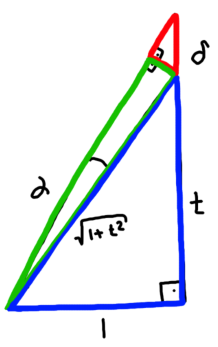
\includegraphics[height=40mm]{pics/atan.pdf}
	\end{block}
\end{frame}

\begin{frame}\frametitle{\mytitle}
	\hfill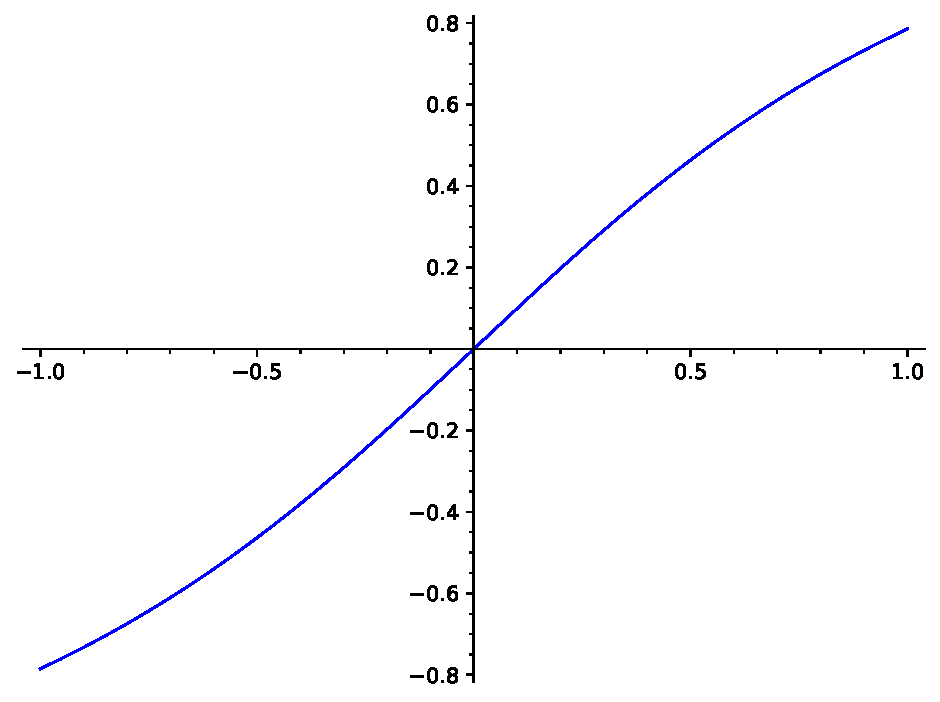
\includegraphics[height=30mm]{pics/plot_atan.pdf}
	\begin{block}{Eigenschaften des arctan}
		\begin{itemize}
			\item Weil $\arctan'(z)>0$, ist die Funktion streng monoton wachsend:
				\begin{align*}
					\arctan(x)>\arctan(y)\quad\mbox{wenn}\quad x>y.
				\end{align*}
			\item Die Funktion ist \emph{ungerade}, d.h.
				\begin{align*}
					\arctan(-x)&=-\arctan(x).
				\end{align*}
		\end{itemize}
	\end{block}
\end{frame}

\begin{frame}\frametitle{\mytitle}
	\begin{block}{Die Kreiszahl $\pi$}
		\begin{itemize}
			\item Wir \emph{definieren}
				\begin{align*}
					\pi&=4\cdot\arctan(1)=\int_0^1\frac{4}{1+x^2}\dd x.
				\end{align*}
			\item {\itshape Intuition: bei gleichen Kathetenl\ae ngen hat ein rechtwinkliges Dreieck einen Winkel von $\pi/4$.}
			\item Weil $1/2\leq 1/(1+z^2)\leq1$ f\ue r $z\in[0,1]$, gilt $2\leq\pi\leq4$.
			\item Durch Ableiten sieht man ferner, da\ss\
				\begin{align*}
					\arctan(z)+\arctan(1/z)&=\frac{\pi}{2}\qquad(z>0).
				\end{align*}
			\item Daraus folgt, da\ss\ $\arctan:\RR\to(-\pi/2,\pi/2)$ bijektiv ist.
		\end{itemize}
	\end{block}
\end{frame}

\begin{frame}\frametitle{\mytitle}
	\hfill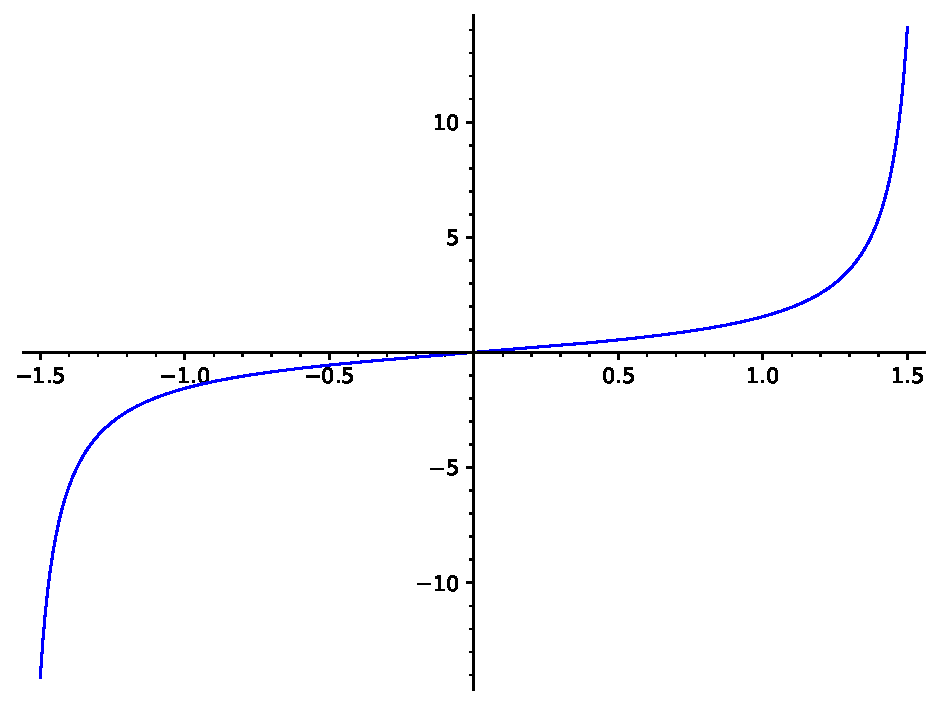
\includegraphics[height=30mm]{pics/plot_tan.pdf}
	\begin{block}{Der Tangens}
		\begin{itemize}
			\item Wir definieren $\tan:(-\pi/2,\pi/2)\to\RR$ als die Umkehrabbildung von $\arctan$.
			\item Diese Funktion setzen wir auf $\RR\setminus\cbc{(2k+1)\pi/2:k\in\ZZ}$ durch
				\begin{align*}
					\tan(x+\pi)=\tan(x)
				\end{align*}
				fort.
		\end{itemize}
	\end{block}
\end{frame}

\begin{frame}\frametitle{\mytitle}
	\begin{block}{Der Tangens (fortgesetzt)}
		\begin{itemize}
			\item Es gilt $\tan(-x)=-\tan(x)$.
			\item Die Abbildung $x\in(-\pi/2,\pi/2)\mapsto\tan(x)$ ist streng monoton wachsend und
				\begin{align*}
					\tan(x)\tan\bc{\frac{\pi}{2}-x}=1.
				\end{align*}
			\item Aus dem Satz \ue ber die Umkehrfunktion folgt
				\begin{align*}
					\tan'(x)=1+\tan^2(x).
				\end{align*}
		\end{itemize}
	\end{block}
\end{frame}

\begin{frame}\frametitle{\mytitle}
	\hfill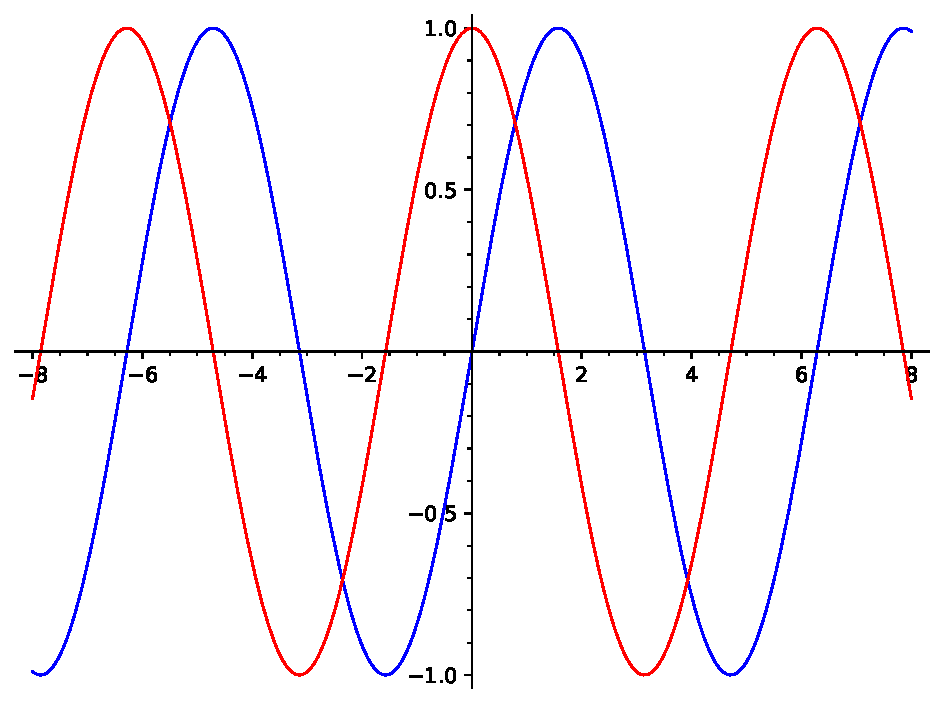
\includegraphics[height=30mm]{pics/plot_sincos.pdf}
	\begin{block}{Sinus und Cosinus}
		\begin{itemize}
			\item Wir \emph{definieren} f\ue r $x\in(-\pi/2,\pi/2)$
				\begin{align*}
					\cos(x)&=\frac{1}{\sqrt{1+\tan^2(x)}}&
						\sin(x)&=\frac{\tan(x)}{\sqrt{1+\tan^2(x)}}
				\end{align*}
			\item Ferner definieren wir
				\begin{align*}
					\cos(\pi/2)&=0&\sin(\pi/2)&=1\\
					\cos(x+\pi)&=-\cos(x)&\sin(x+\pi)&=-\sin(x)
				\end{align*}
		\end{itemize}
	\end{block}
\end{frame}

\begin{frame}\frametitle{\mytitle}
	\begin{block}{Sinus und Cosinus (fortgesetzt)}
		\begin{itemize}
			\item Es gelten die Gleichungen
				\begin{align*}
					\cos(-x)&=\cos(x)&\sin(-x)&=-\sin(x)\\
					cos(x+2\pi)&=\cos(x)&\sin(x+2\pi)&=\sin(x)
				\end{align*}
			\item F\ue r die Ableitungen gilt
				\begin{align*}
					\sin'(x)&=\cos(x)&\cos'(x)&=-\sin(x)
				\end{align*}
		\end{itemize}
	\end{block}
\end{frame}

\begin{frame}\frametitle{\mytitle}
	\begin{block}{Sinus und Cosinus (fortgesetzt)}
		\begin{itemize}
			\item Unmittelbar aus den Definitionen und mittels der Ableitung folgt die Gleichung
				\begin{align*}
					\sin^2(x)+\cos^2(x)=1.
				\end{align*}
			\item Ebenfalls durch Ableiten erhalten wir die \alert{Additionstheoreme}:
				\begin{align*}
					\sin(x+y)&=\sin(x)\cos(y)+\cos(x)\sin(y)\\
					\cos(x+y)&=\cos(x)\cos(y)-\sin(x)\sin(y)
				\end{align*}
		\end{itemize}
	\end{block}
\end{frame}

\begin{frame}\frametitle{\mytitle}
	\begin{block}{Zusammenfassung}
		\begin{itemize}
			\item Auf dem Weg \ue ber den $\arctan$ haben wir die trigonometrischen Funktionen eingef\ue hrt.
			\item Mittels der Differential- und Integralrechnung konnten wir die bekannten Eigenschaften dieser Funktionen herleiten.
		\end{itemize}
	\end{block}
\end{frame}



\end{document}
